\chapter[Desenvolvimento ]{Desenvolvimento}
Neste projeto foi acordado o Desenvolvimento da tecnologia de Manutenção Remota envolvido no projeto de gestão de embarcados dos ATM’s e TFL’s.

\section{Verifica\c{c}\~ao de Informa\c{c}\~oes}

\bigskip

{\color{black}
    \ \ \ \ O processo de obten\c{c}\~ao de informa\c{c}\~oes das m\'aquinas da Caixa Econ\^omica Federal sempre foi feita
        de maneira manual, utilizando shell scritps. Foi proposto e implantado o desenvolvimento de um painel de
        monitora\c{c}\~ao e manuten\c{c}\~ao remota dos equipamentos. O primeiro ponto para que a solu\c{c}\~ao fosse
        satisfeita foi executar a manuten\c{c}\~ao remota, resgatando as informa\c{c}\~oes de uma determinada m\'aquina. }

{\color{black}
    \ \ \ \ Primeiramente, o usu\'ario dever\'a indicar qual a ag\^encia que pertence a m\'aquina que \ est\'a sujeita ao
        recolhimento de dados, logo em seguida, escolhendo-a. Est\~ao a a\c{c}\~ao de recupera\c{c}\~ao de informa\c{c}\~oes
        pode ser feita com o seguinte bot\~ao no painel:}

        \begin{center}
        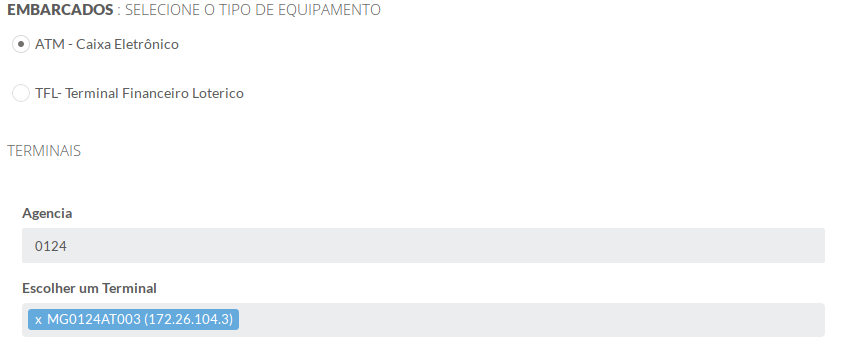
\includegraphics[width=17.029cm,height=7.22cm]{figuras/RATCETECATMSTFLS051718v2-img002.png}
        \end{center}


        \begin{center}
        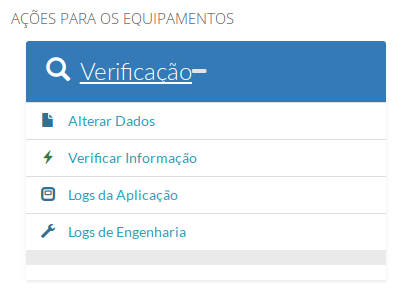
\includegraphics[width=10.82cm,height=7.777cm]{figuras/RATCETECATMSTFLS051718v2-img003.png}
        \end{center}
{\color{black}
    \ \ \ \ Dessa forma, ao solicitar a verifica\c{c}\~ao de informa\c{c}\~oes, o servidor ir\'a recuperar os dados
        atrav\'es do servi\c{c}o ssh na m\'aquina. Ele ir\'a levantar todas as informa\c{c}\~oes e ir\'a apresentar as suas
        informa\c{c}\~oes ao usu\'ario. As informa\c{c}\~oes coletadas ser\~ao as seguintes:}


        \bigskip

{\color{black}
    \ \ }

    \begin{center}
    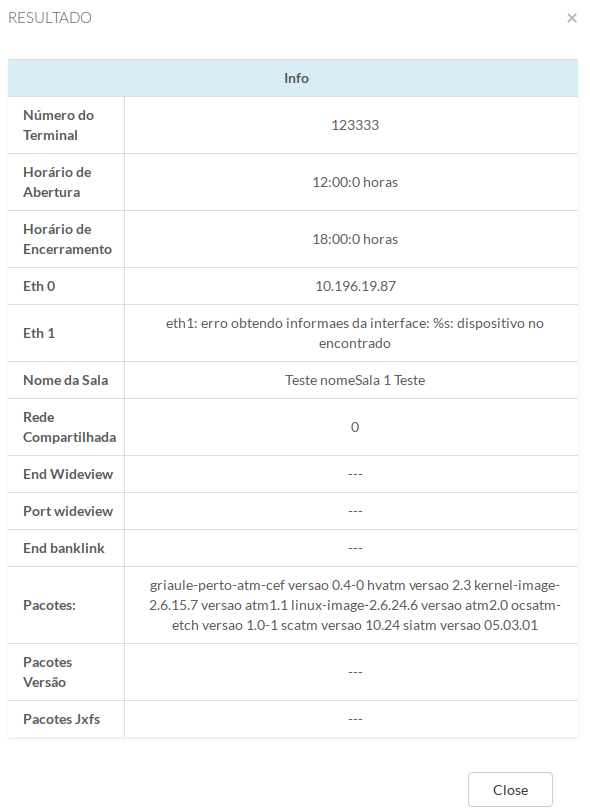
\includegraphics[width=13.936cm,height=19.131cm]{figuras/RATCETECATMSTFLS051718v2-img004.png}
    \end{center}

    \bigskip


    \bigskip

    \section[\ \ Altera\c{c}\~ao de Dados]{\ \ Altera\c{c}\~ao de Dados}
{\color{black}
    \ \ Para a aplica\c{c}\~ao de altera\c{c}\~ao de dados, no momento, \'e apresentado um formul\'ario que possibilita a
        altera\c{c}\~ao de dados j\'a existentes. Para aplicar uma altera\c{c}\~ao de dados, \'e necess\'ario escolher a
        m\'aquina que receber\'a a mudan\c{c}a.}

{\color{black}
    \ \ Ao escolher o terminal, \'e poss\'ivel selecionar a op\c{c}\~ao para executar a altera\c{c}\~ao, como visto na
        representa\c{c}\~ao a seguir:}

{\color{black}
    \ \ \ \ Sendo selecionada a op\c{c}\~ao, ser\'a apresentado ao usu\'ario o formul\'ario, como dito acima:}

    \begin{center}
    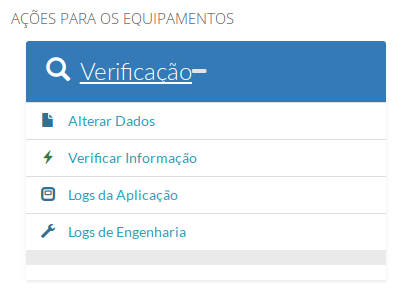
\includegraphics[width=10.82cm,height=7.777cm]{figuras/RATCETECATMSTFLS051718v2-img005.png}
    \end{center}

    \bigskip

{\color{black}
    \ \ Ap\'os o preenchimento do formul\'ario com as devidas informa\c{c}\~oes, estas ser\~ao enviadas para o servidor e
        aplicadas na respectiva m\'aquina. Assim, ir\'a ser criada uma barra de carregamento na parte inferior do site que
        apontar\'a o status atual da tarefa, sendo em progresso ou conclu\'ido. }

        \begin{center}
        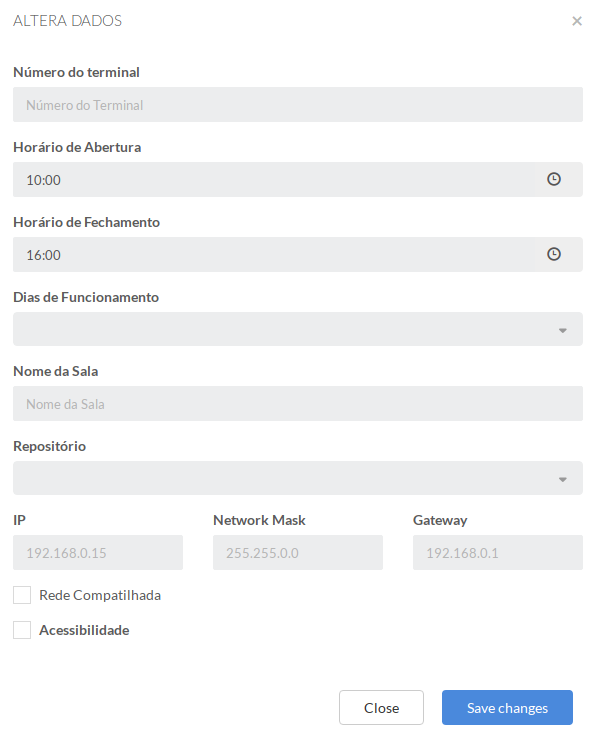
\includegraphics[width=15.279cm,height=18.83cm]{figuras/RATCETECATMSTFLS051718v2-img006.png}
        \end{center}

        \bigskip


        \bigskip


        \bigskip

{\color{black}
    \ \ Ao ter a tarefa finalizada, ser\'a apresentado o status de conclu\'ido e de visualiza\c{c}\~ao dos logs.}

    \begin{center}
    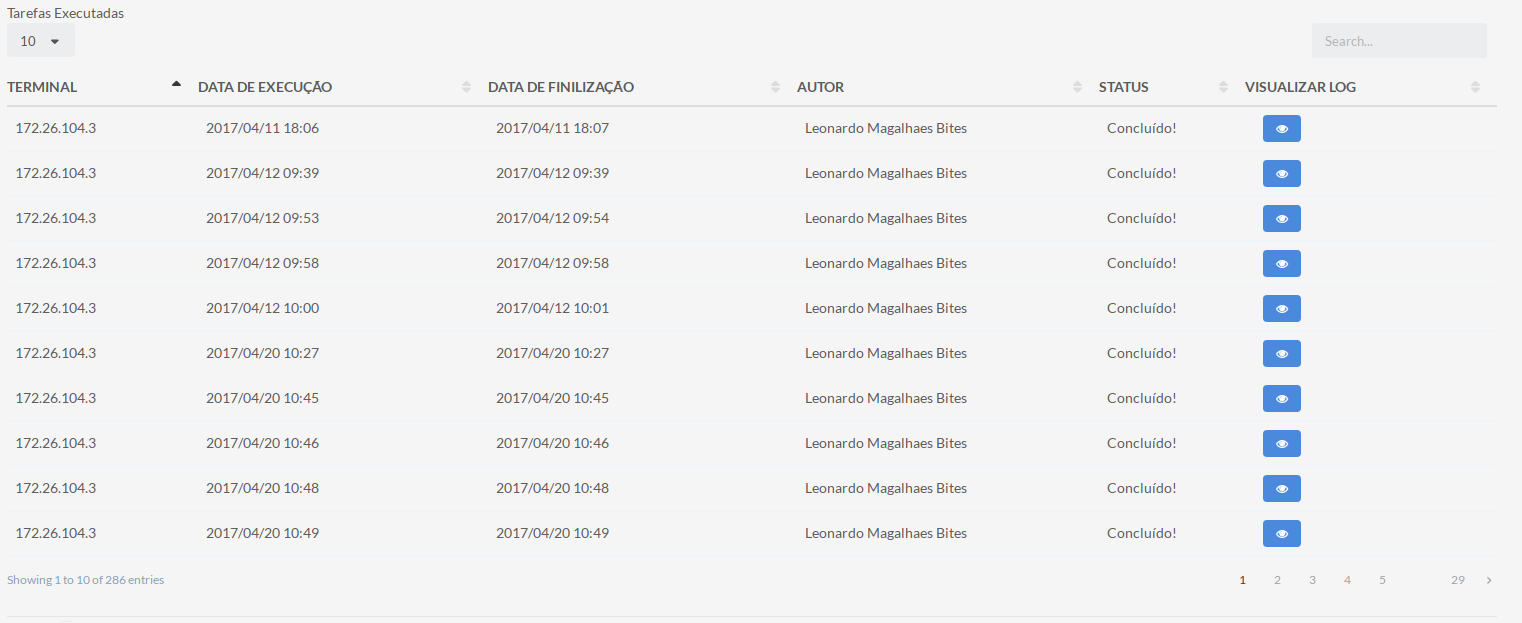
\includegraphics[width=17.029cm,height=6.969cm]{figuras/RATCETECATMSTFLS051718v2-img007.png}
    \end{center}

    \bigskip

    \section{Salvar Logs}
{\color{black}
    \ \ A funcionalidade de salvar log tem como objetivo principal recuperar dois tipos de logs dos terminais. O primeiro
        deles s\~ao os logs da aplica\c{c}\~ao SIMMA, sendo que o segundo s\~ao os logs de engenharia. }

{\color{black}
    \ \ Ap\'os escolher o terminal, que ter\'a o log recolhido, existem duas op\c{c}\~oes para a recupera\c{c}\~ao dos logs,
        como dito a pouco. Estas est\~ao dispostas como exemplificado na tela a seguir:}


        \bigskip

{\color{black}
    \ \ Ao solicitar uma das duas aplica\c{c}\~oes de logs, ser\'a enviada uma solicita\c{c}\~ao para as m\'aquinas, que
        ir\~ao armazenar os dados e enviar para o site. Assim, ser\'a indicado na barra de status, mencionada a pouco, que foi
        finalizada a tarefa com sinal de conclu\'ida. O usu\'ario dever\'a selecionar a op\c{c}\~ao de visualizar log e, logo
        em seguir, baixar o log. }

        \begin{center}
        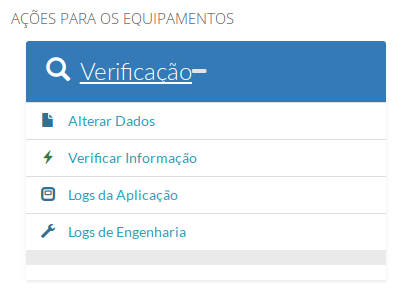
\includegraphics[width=10.82cm,height=7.777cm]{figuras/RATCETECATMSTFLS051718v2-img008.png}
        \end{center}

        \bigskip

        \section{Manuten\c{c}\~ao}
{\color{black}
    \ \ A manuten\c{c}\~ao permite que os terminais tenham manuten\c{c}\~oes pr\'e definidas. Estas podem ser aplicadas em
        v\'arios terminais ao mesmo tempo. \ Estes terminais devem ser escolhidos e assim, podem ser abordadas as
        manuten\c{c}\~oes, que est\~ao dispon\'iveis de acordo com a imagem do servidor a seguir:}


        \bigskip

        \section[Aspectos T\'ecnicos]{Aspectos T\'ecnicos}
        \begin{center}
        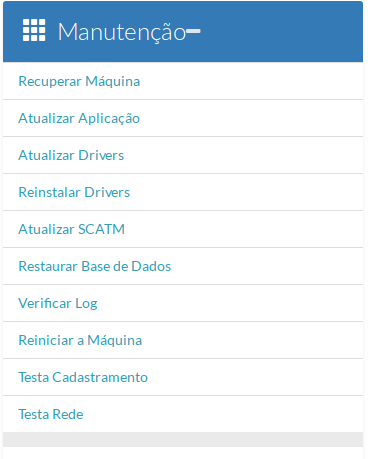
\includegraphics[width=9.793cm,height=12.143cm]{figuras/RATCETECATMSTFLS051718v2-img009.png}
        \end{center}
{\color{black}
    \ \ A seguir ser\~ao apresentados os procedimentos sistem\'aticos, que foram implementados para possibilitar o
        cumprimento dos requisitos desejados pelo cliente. Os cap\'itulos a seguir ser\~ao divididos bem como a arquitetura do
        software. O primeiro cap\'itulo ir\'a apresentar a parte de apresenta\c{c}\~ao, bem como HTML, CSS e JS. O segundo
        cap\'itulo apresentar\'a as views, que fazem e exercem o controle dos procedimentos solicitados ao servidor. Por fim,
        ser\~ao apresentados os procedimentos de implementa\c{c}\~ao nas modelos e scripts de execu\c{c}\~ao. }


        \section[Camada de Apresenta\c{c}\~ao]{Camada de Apresenta\c{c}\~ao}
{\color{black}
    A seguir ser\~ao apresentados os c\'odigos procedurais de apresenta\c{c}\~ao do site. O primeiro apresentado ser\'a a
        tela de index.html da tela de manuten\c{c}\~ao.} Os códigos estão no Anexo \ref{ane:um}.

        

    \section{Camada de Controle dos Dados}
{\color{black}
    Nos scripts a seguir, ser\~ao apresentados todos os procedimentos do servidor que manipulam o controle e direcionamento
        dos dados.}

{\color{black}
    O primeiro a ser apresentado ser\'a o arquivivo de views.py:}
Os códigos estão no Anexo \ref{ane:dois}.

    \section{Camada de Execu\c{c}\~ao}
{\color{black}
    Ser\~ao apresentados todos os scripts para a implementa\c{c}\~ao de aplica\c{c}\~ao de altera\c{c}\~oes de dados nas
        m\'aquinas.}

{\color{black}
    O primeiro apresentado, ser\'a a modelo de heran\c{c}a, como base para todos os outros comandos.}
Os códigos estão no Anexo \ref{ane:tres}.

    \section{Execu\c{c}\~ao dos Servi\c{c}os}
{\color{black}
    Para iniciar a aplica\c{c}\~ao, \'e necess\'ario apenas executar o comando de start da aplica\c{c}\~ao:}

{\ttfamily\color[rgb]{0.10980392,0.10980392,0.10980392}
    python run.py}
